%!TEX Root = main.tex

%\section{Blob analysis details}\label{sec:blob_analysis}

%This section describes in details the basic blob analysis performed on FPGA framegrabber using the library provided by Silicon Software GmbH. For more detailed information an application note from \cite{blob_analysis} is recommended. 
%
%The 8 bit gray scale image is transformed into a black/white (0/1) image. There are two basic binarization methods implemented in the blob recorder. First is a simple thresholding, such that all the pixels with values above a user-selected threshold turn into white (1), and the rest become black (0) and are removed from the following analysis. A more complex adaptive local thresholding is implemented for the cases of non-uniform illumination, for which the background cannot be segmented out using a single threshold.

%\begin{figure}[!ht]
%\centering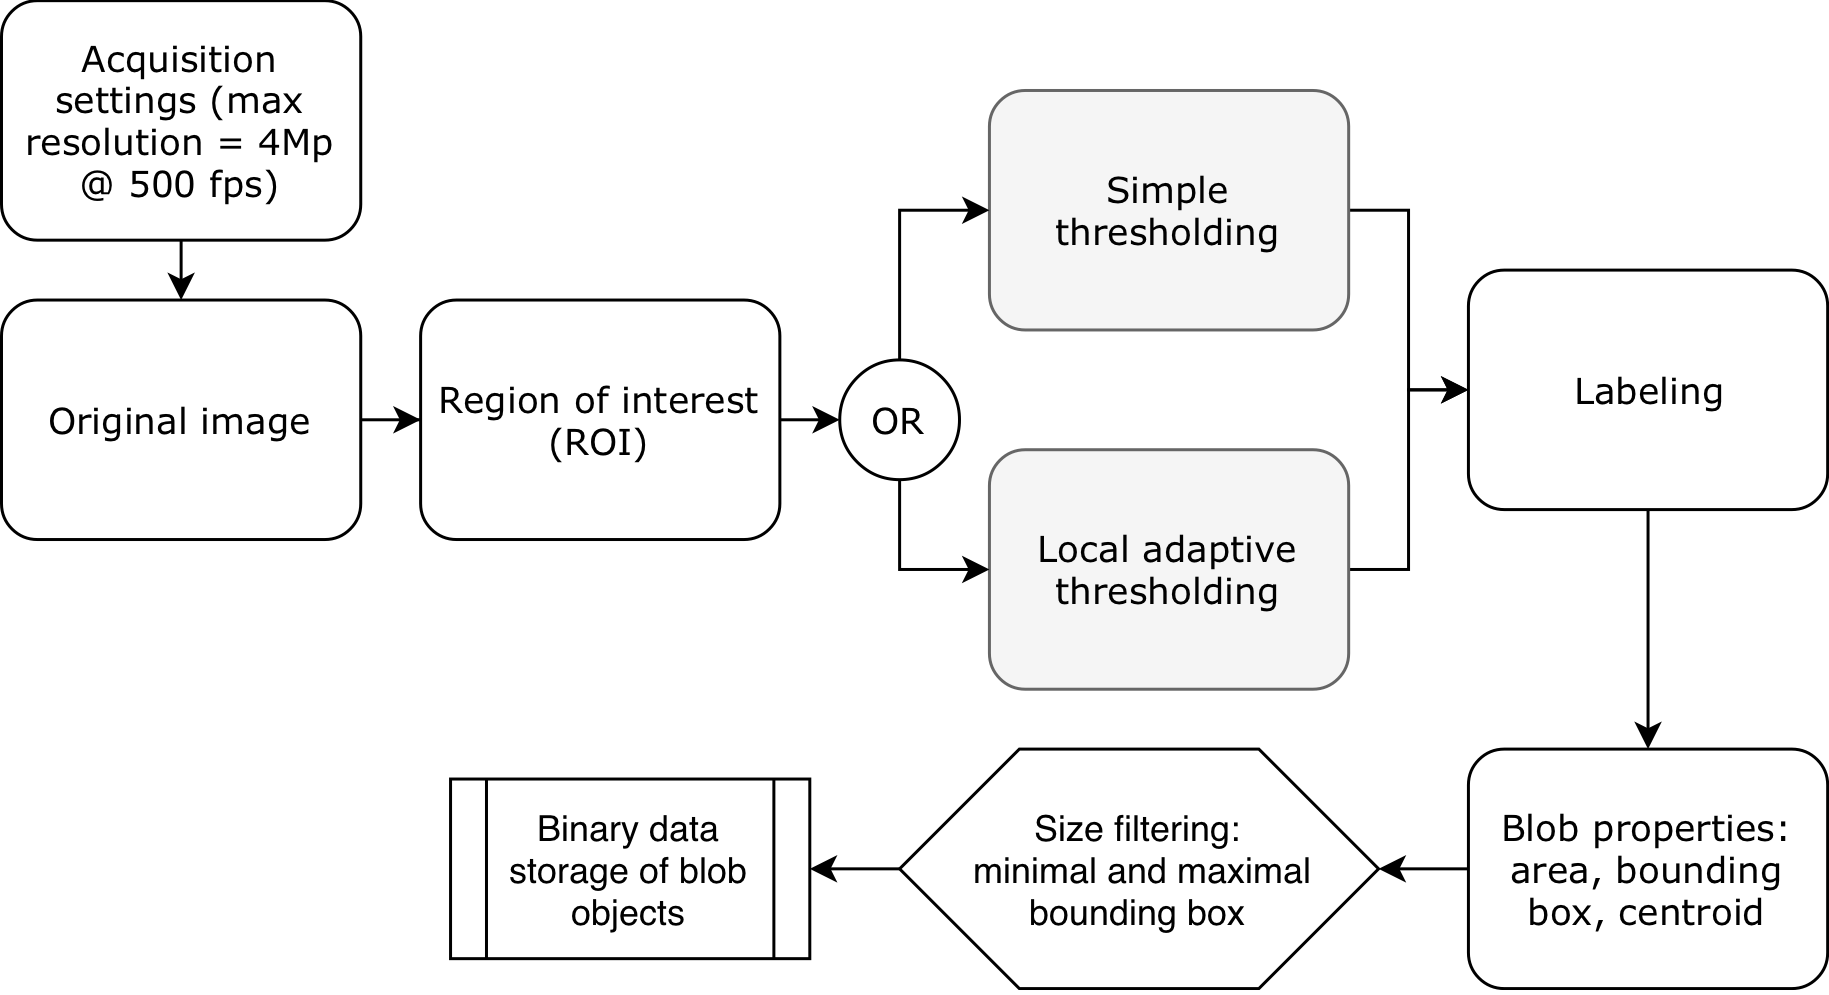
\includegraphics[width=.9\textwidth]{draw.io/blob_analysis.pdf}
%\caption{Diagram of the blob analysis algorithm. \label{fig:blob_analysis}}
%\end{figure}

%The adaptive local thresholding is based on the xxx\cite{xxx}. The key parameters are the size of the window for which a local histogram is estimated, minimum and maximum values for the difference between the background and the foreground (object). 
%
%The following step is labeling of the detected objects (blobs) and filtering them by size. Two size thresholds, the minimum and maximum allowable sizes are provided by the user and only the objects within a given range of sizes are preserved. 



% \subsection{Blob recorder with examples}

% TAU Algorithm Description - Blob Analysis on FPGA 
% Written by: Erez Shapira, 26/04/2018
%In the following description, the notation $(i,j)$ refers to pixel location in image coordinates. Column location ($x$-axis) is $i$ in range $[0, M-1]$, where $M$ is the width, and row location $(y-axis)$ is $j$ in range $[0, N-1]$ where $N$ is the height of the image. $(i,j)=(0,0)$ refers to the top-left corner of the image.
%
%The algorithm stages depicted below are presented in the same order that they are performed, so generally the output of each stage is fed as an input to the next stage.
%
%\begin{itemize}
%	\item \textbf{Streaming input} The recording system is based on four CMOS cameras (Optronis GmbH) that transfer data to the frame-grabber. It uses the  CoaXPress (CXP) protocol in 4 lanes, each up to 6.25 Gbit/sec, at a maximal total bandwidth of 25 Gbit/sec. The camera resolution is $ 2304 \times 1720$  ($M \times N$) at frame rates up to 500 Hz (frames per second). All further image processing is performed in real-time on the entire input stream, at full frame rate of the camera. An example of the input image is shown in Fig.~\ref{fig:blob_example}a (only a small region of 256 $\times$ 256 pixels is shown for the sake of brevity).
%% 
%\item \textbf{Input buffer} – Image data buffering is preformed with 2 parallel high-speed DDR3 memory banks. Each memory bank is 256 MByte, with data bandwidth of 3.2 GByte/sec. When there is momentary load on image processing engine or on image transfer, the image data is accumulated on the input buffer without losing data.
%%
%	\[ P(i,j)\textsubscript{out} = P(i,j)\textsubscript{in} \]
%%
%\item \textbf{8-bit Lookup Table (LUT)}: Each 8-bit input grey value is mapped to another 8-bit value, using some pre-defined lookup table. This can be used for performing digital gain or any other arithmetic function on input grey values.
%
%\[ P(i,j)\textsubscript{out} = \mathrm{LUT}(P(i,j)\textsubscript{in}) \]
%\noindent where LUT($x$) is the lookup table's output value for entry $x$. Both $x$ and LUT($x$) are integer values in range [0, 255]. Default mapping is identity mapping: 
%\[ \mathrm{LUT}(x) = x \]
%%
%\item \textbf{Median Filter} is an optional step that can be turned on/off by the user, where each pixel is replaced by the median of $ 3 \times 3$ neighboring pixels. In our application it helps to remove small noisy areas, typically sized 1-2 pixels.

%\begin{frame}
%\[ P(i,j)\textsubscript{out} = \mathrm{median}  
%\begin{bmatrix}
% P(i-1, j-1) &  P(i, j-1) & P(i+1, j-1) \\
%P(i-1, j) &  P(i, j) & P(i+1, j) \\
%P(i-1, j+1) & P(i, j+1)& P(i+1, j+1)
%\end{bmatrix}_\textrm{in}
%\]
%\end{frame}

%\item \textbf{Background subtraction}: A pre-defined background image can be loaded into this operator. This background image is stored in 2 parallel high-speed DDR3 memory banks. Then for each new frame, the background image is read from memory and subtracted from the input image, pixel-by-pixel. This allows removing of any constant spatial noise and unwanted light reflections from the image scene.
%%
%\[  P(i,j)\textsubscript{out} = \max(0, (P(i,j)\textsubscript{in} - P(i,j)\textsubscript{background})) \]
%%
%\item \textbf{Offline image injection}: An offline image from pre-recorded file can be injected into the algorithm instead of the camera input image. This can be used for testing a known image with various parameter values, and for adjusting the algorithm parameters. When offline image is injected, the background subtraction cannot be performed, since both operators are sharing the same physical memory banks.
%%
%\[  P(i,j)\textsubscript{out} = P(i,j)\textsubscript{offline}\]
%%
%\item \textbf{Polarity Inversion} [optional]: This optional operation inverts each pixel's grey level, for instance in shadow imaging PTV when the system locates dark objects on a bright background. The inversion is required since the following segmentation algorithm is designed to find bright objects on a dark background. This operation can be skipped if not required.
%%
%\[ P(i,j)\textsubscript{out} = 255 - P(i,j)\textsubscript{in} \]
%%
%\item \textbf{Binarization}

%\begin{itemize}
%\item {\bf Local adaptive threshold}: the input image is binarized by comparing each pixel to the average of its surrounding pixels:  
%%
%\begin{enumerate} 
%\item First, for each pixel, a local average of the surrounding kernel of a pre-defined size, e.g. $8 \times 8$ (presently 8, 16 and 32 pixel$^2$ kernels are implemented but pixels are diluted to $8 \times 8$ values) pixels is computed. A positive offset may be added to the average.
%
%\[  A \left( i,j \right) =  \mathrm{Offset} + \sum\limits_{m=i-4}^{i+3} \; \sum\limits_{n=j-4}^{j+3}P \left( m,n \right) _\mathrm{in}   \]
%
%\item Then each pixel value is compared against the value of its local average plus the offset, $A(i,j)$. If the difference is greater or equal to a pre-defined threshold $T_\mathrm{diff}$, or pixel value itself is is greater or equal to some absolute threshold $T_\mathrm{fixed}$, then the pixel marked as bright pixel (1). Otherwise the pixel is marked as dark pixel (zero or background).
%\end{enumerate}
%
%\[ 
%P(i,j)\textsubscript{in} -  A(i,j)  \geq   T\textsubscript{diff} \lor  P(i,j)\textsubscript{in}  \geq  T\textsubscript{fixed} \Rightarrow  P(i,j)\textsubscript{out }= 1
%\]
%
%\item \textbf{Fixed threshold}: An alternative image binarization method compares each pixel to some pre-defined fixed threshold, $T_\mathrm{fixed}$:
%
%\[ P(i,j)\textsubscript{in} \geq   T\textsubscript{fixed}  \Rightarrow P(i,j)\textsubscript{out }=\ 1  \]
%
%\end{itemize}
%%
%\item \textbf{Image output}: There is an option to store the output image $P_\mathrm{out}$ to the host PC memory for display or further off-line image processing. In order to decrease system load, the operator can output $N$ image in range [1, 511]. For debugging purposes the output image can be stored before or after binarization stage (converted from [0,1] to [0,255] range). An example of the binarized image is shown in Fig.~\ref{fig:blob_analysis}b. 
%%
%%\begin{itemize}
%%	\item P(i,j)\textsubscript{out }= P(i.j)\textsubscript{grey}\  , OR:\par
%%
%%P(i,j)\textsubscript{out }= 255 x P(i.j)\textsubscript{binarized}\par
%%
%
%\item \textbf{Segmentation using blob analysis}: A rectangular region of interest (ROI) from the binary image is passed to segmentation and blob analysis. Note that if necessary the image resolution can be reduced, which then allows a significant increase of the data acquisition rate (see Fig.~\ref{fig:blob_analysis}).
%
%Blob analysis algorithm locates and measures connected regions of bright pixels (called blobs), and outputs information on each one of the connected regions  for further analysis of the scene. The data output on each blob includes area in pixels, center of gravity coordinates and enclosing rectangle coordinates. The center of gravity coordinates are given at resolution of $1/256$ pixel. All coordinates are relative to image top-left corner. The current implemented algorithm uses 8-connected objects, but it can be easily modified to find 4-connected objects. Detailed information on implementation of blob analysis operator in FPGA is provided by the framegrabber manufacturer~\cite{blob_analysis}. The result can be displayed on an original image as marked blobs, see Fig.~\ref{fig:blob_analysis}c. 
%
%% \href{http://www.siliconsoftware.de/download/live\_docu/VA3/en/app\_notes/sug012\_va\_BlobAnalysis.pdf}{http://www.siliconsoftware.de/download/live\_docu/VA3/en/app\_notes/sug012\_va\_BlobAnalysis.pdf}\par
%\item \textbf{Objects filtering and output}: The blobs are optionally filtered by area and only blobs in range [area\textsubscript{min}, area\textsubscript{max}] are stored to the host PC. This stage can remove very small objects, which can be considered as noise, and also very large objects, such as background light reflected on image.
%\end{itemize}

\begin{frame}
\begin{card}
\centering
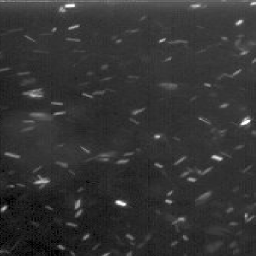
\includegraphics[width=.3\textwidth]{1_in}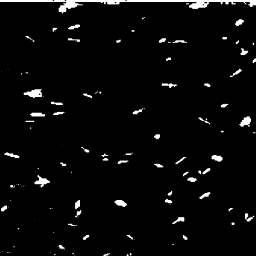
\includegraphics[width=.3\textwidth]{1_binarized}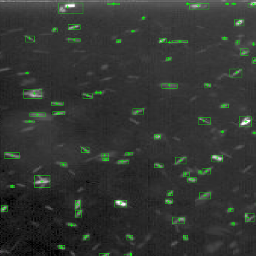
\includegraphics[width=.3\textwidth]{1_out}
\end{card}
\vspace{-.5cm}
\begin{cardTiny}
An example of a raw 3D-PTV image from laboratory experiment \cite{Kreizer2011}. (a) Original image example, (b) binarized image, (c) blobs marked on the original image. This example is using median filter, without polarity inversion, an adaptive filter with the offset of 20, $T_\mathrm{diff} = 0$, $T_\mathrm{fixed} = 90$ and filtering out blobs smaller than 20 pixels.  
\end{cardTiny}
\end{frame}


\begin{frame}
\begin{card}
\centering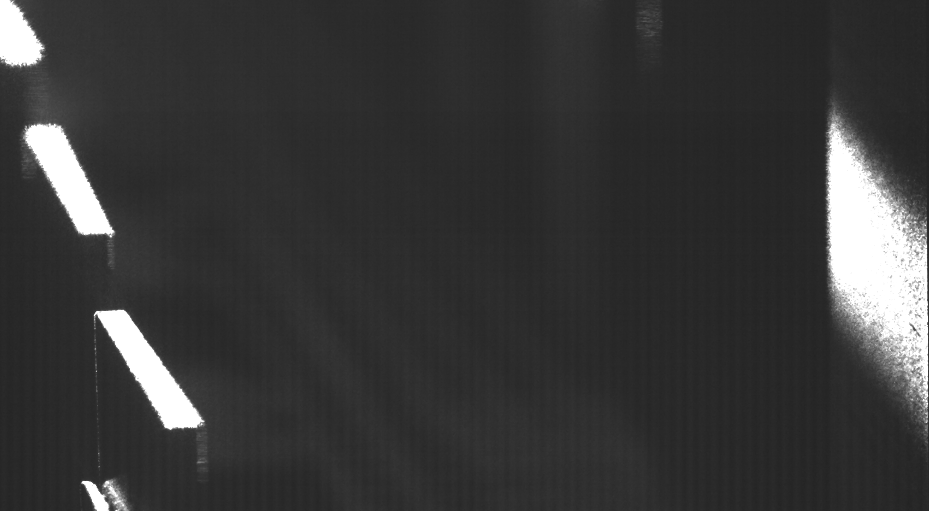
\includegraphics[width=.45\textwidth]{background.png} \hspace{.5cm}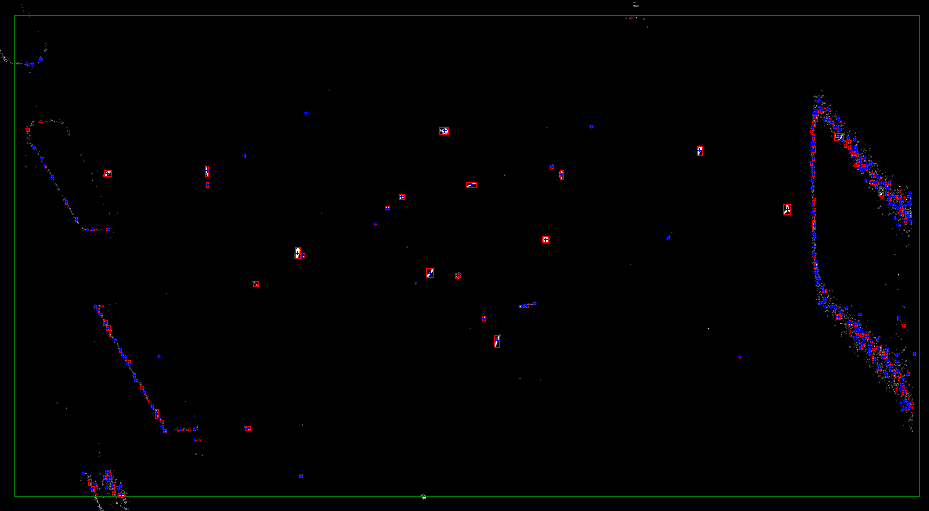
\includegraphics[width=.45\textwidth]{detection.png} \hspace{.5cm} 
\end{card}
\begin{card}
An example of a raw 3D-PTV image the wind tunnel experiment. (a) Background image with no particles, (b) binary image after background subtraction, and detection using a local filter 
\end{card}
\end{frame}
%- Processed with applet "Blob_2D_30_8x8.hap"
%- Parameters:
%	Noise removal = enabled
%	Polarity inversion = disabled
%	Threshold method = adpative
%	Threshold offset = 20
%	Threshold diff = 0
%	Bright level threshold = 90
%	Area min = 20
%	Area max = 10000


%The data compression ratio is significantly larger than typical real-time image processing routines for PIV or PTV \cite{Kreizer2011}. At 25 Gbit/sec the input stream can be recorded to the RAM of the host PC for several seconds. Although this is a possible solution for short recordings, calibration or adjustment of parameters (saving offline or background images), the wind tunnel measurements require continuous recording to enable tracking at full speed and intermittently when the seeding creates an acceptable particle images quantity and quality. The processed data of blobs is stored at roughly $\sim 1/1000$ compression ratio. 











